\documentclass[11pt]{beamer}
\usepackage[utf8]{inputenc}
\usepackage[T1]{fontenc}
%\usepackage{natbib}
\usetheme{Pittsburgh}
\usepackage{verbatim} 
\usepackage{multicol}
\usepackage[english]{babel}
\usepackage{epstopdf}
\setbeamercolor{block body}{bg=green!10}
\setbeamertemplate{blocks}[rounded]%[shadow]
%\titlegraphic{\vspace*{1cm}
	%\includegraphics[width=3cm]{figuras/uniss.png}
	%\hspace*{1cm}~%
%		\includegraphics[width=3.5cm]{logo_FCEA.png}
%}
\setbeamertemplate{navigation symbols}{}
\setbeamertemplate{footline}[frame number]
\AtBeginSection{ 
	\begin{frame}
		\frametitle{Index}
			\tableofcontents[currentsection]
	\end{frame}
}
\begin{document}
	\title{Modelos dinámicos y computacionales en Economía}
	\subtitle{Modelos Basados en Agentes y Metodología}
	%\logo{}
	\institute{Licenciatura en Economía, FCEA, UDELAR}
	\date{7 de noviembre de 2023}

	%\subject{}
	%\setbeamercovered{transparent}
	%\setbeamertemplate{navigation symbols}{}
	\frame[plain]{
	\begin{figure}
	\centering
	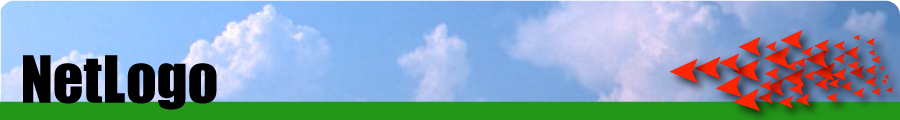
\includegraphics[width=0.7\linewidth]{figuras/netlogo-title-wide-60.jpg}
	%		\caption{}
	\label{fig:netlogo-title-wide-60}
\end{figure}	
		\vspace{-1cm}
\maketitle
}

\begin{frame}
\frametitle{Contenido de la clase:}
\begin{itemize}
	\item Complejidad
 \item Modelos Basados en Agentes (ABM)
 \item Economía de la Complejidad y Agent-Based Computational Economics (ACE)
 \item Metodología para ABM
\end{itemize}
\end{frame}

\begin{frame}
	\frametitle{Complejidad}
 \framesubtitle{Introducción}
\begin{itemize}
\small \item Muchos fenómenos no pueden ser explicados con conceptos de física mecánica.
\item Las estructuras grandes se ensamblan a partir de partículas o individuos de una manera mucho más allá de la simple agregación y suma.
\item Estructuras evolucionan hacia un futuro y formas impredecibles.
\item La flecha del tiempo no es reversible y muchos métodos científicos tradicionales fallan en su explicación y pronóstico.
\item Comúnmente los sistemas presentan heterogeneidad y producen innovaciones.
\item El sistema (sociedad) está poblado por agentes heterogéneos que interactúan con los demás.
\item Estamos lejos de comprender el Mundo o la Realidad con la máquina newtoniana o el punto de vista estadístico, principalmente en las ciencias sociales y económicas.
\end{itemize}

\end{frame}

\begin{frame}
\frametitle{Complejidad}
\framesubtitle{¿Qué implica \textit{complejidad}?}
\hline
\begin{quote}
\footnotesize    ``An \textbf{interdisciplinary} field of research that seeks to explain how \textbf{large} number of relatively \textbf{simple} entities \textbf{organize themselves}, \underline{without the benefit of any central controller} into a collective whole that creates \textbf{patterns}, uses information, and, in some cases, \textbf{evolves} and \textbf{learns}.'' (Mitchell, 2009)
\end{quote}
\hline
\begin{quote}
 \footnotesize   \textcolor{blue}{``A \textbf{system of connected agents} that exhibits an \textbf{emergent} global behavior \underline{not imposed by a central controller}, but resulting from the \textbf{interactions} between agents.'' (Boccara, 2004, p.4)}
\end{quote}
\hline
\begin{quote}
 \footnotesize   ``Complex systems consist of units \textbf{interacting} in a \textbf{hierarchy} of levels, including \textbf{subsystems} composed of even more intricate sub-subsystems. Complex systems exhibit \textbf{emergent properties} due to the \textbf{interaction} of their subsystems when certain unspecific environmental conditions are met, and they show \textbf{temporal and/or spatial patterns} on a scale that is orders of magnitude bigger than the scale on which the subsystems interact.'' (Fuchs 2013, p.4)
\end{quote}
\hline
\begin{quote}
 \footnotesize  \textcolor{blue}{``The science of complexity suggests that while life is in accordance with the laws of physics, physics cannot predict life.'' (Erdi, 2008)}
\end{quote}    
\hline


\begin{comment}
    \begin{frame}
\frametitle{Complexity}
\framesubtitle{Some important aspects}
\begin{itemize}
\item Diversity/variety
\item High Non-linearity
\item Hierarchy
\item Non-Predictability
\item Interactions (at micro and macro
level)
\item Network
\item Self organization
\item Adaptive system
\item Emergence
\item Learning and information
computation
\item Evolution
\end{itemize}
\end{frame}
\end{comment}


\begin{frame}{Enfoques de la complejidad}
\begin{enumerate}
\item \small Sistema no lineal de ecuaciones diferenciales (a nivel macro)
\begin{itemize}
 \footnotesize   \item Inestabilidad 
 \item Equilibrios múltiples 
 \item Replicador dinámico o sistema Lotka-Volterra 
 \item Bifurcación 
 \item Caos determinista 
 \item Estructuras fractales
\end{itemize}
\item Modelos basados en agentes con interacciones
\begin{itemize}
\footnotesize    \item Algoritmos genéticos
     \item Autómatas celulares
     \item Redes
     \item Modelos espaciales
     \item Modelos micro-macro 
\end{itemize}
\item Evolución, Sistema Adaptativo y Cómputo
\begin{itemize}
\footnotesize    \item Información
     \item Cambio individual
     \item Cambio estructural
     \item \textit{Path-dependence} y causalidad acumulativa
     \item Auto-organización (del caos al orden)
\end{itemize}
\end{enumerate}
\end{frame}

\begin{frame}{Modelos Basados en Agentes}
\framesubtitle{Introducción}
 \begin{itemize}
 \small    \item La mayoría de los modelos en Economía se basan en la evolución de cantidades agregadas o promedio.
      \item No hay heterogeneidad ni interacciones presentes.
      \item En el mundo basado en agentes, el comportamiento de un agente tiene un efecto sobre los demás, y el individuo que sigue una regla simple y particular puede producir efectos agregados sorprendentes.
\item Los individuos siguiendo su regla simple particular o colectiva generan una realidad social o económica, observada y analizada por los métodos tradicionales: econometría y modelos estructurales.
\item El investigador (agregado) no puede responder adecuadamente a la pregunta: ¿De dónde viene este patrón agregado?
\item Para responder a esto se necesita un  mundo (modelo) basado en agentes habitado por agentes heterogéneos más que por individuos representativos.
 \end{itemize}
\end{frame}

\begin{frame}{Modelos Basados en Agentes}
\framesubtitle{¿Por qué hacer simulaciones?}
Para analizar problemas sociales complejos (es decir, la evolución de las normas sociales, el desarrollo o la sostenibilidad ambiental) necesitamos una clase diferente de modelos que puedan
  \begin{itemize}
      \item Agregar suposiciones realistas en modelos micro y macro:
incertidumbre, decisiones secuenciales, heterogeneidad, interacciones locales, no equilibrio
\item Replicar parte de la evidencia empírica
\item Incluir cambios estructurales
\item No asumir dinámicas ``macro''.
 \end{itemize}
\end{frame}

\begin{frame}{Modelos Basados en Agentes}
\framesubtitle{¿Por qué hacer simulaciones?}
\begin{itemize}
     \item Interacción de objetos (agentes) como un problema complejo $\rightarrow$ sin solución analítica.
\item La interacción social como un problema complejo (menos sencillo que el comportamiento de los sistemas físicos)
\begin{itemize}
     \item Sin sistema cerrado
\item Interacción de heurísticas y reacciones
\end{itemize}
\item “I can calculate the motion of heavenly bodies, but not the madness of people” (I. Newton)
\item Las interacciones simples pueden conducir a resultados complejos (Arthur, 1994; Schelling, 1971)
\begin{itemize}
\item ```Minority games'', segregación urbana, elección de una tecnología.
\item El lugar del salón donde están sentados ahora
\end{itemize}
 \end{itemize}   
\end{frame}

\begin{frame}{Modelos Basados en Agentes}
\framesubtitle{Agent-Based (Computational) Economics}
\begin{block}{}
 Agent–Based Computational Economics (ACE): “the computational study of
economic processes modelled as dynamic systems of interacting
agents” 
  \vskip5mm
  \hspace*\fill{\small (L. Tesfatsion)}
\end{block} 
\begin{itemize}
 \small   \item El modelador construye un mundo ``económico'' virtual poblado por varios tipos de agentes (económicos, institucionales, sociales, biológicos, físicos)
\item El modelador establece las condiciones iniciales
\item El modelador luego da un paso atrás para observar cómo se desarrolla el mundo en el tiempo (no se permite ninguna otra intervención por parte del modelador)
\item Los eventos son impulsados por las interacciones de los agentes
\end{itemize}
\end{frame}

\begin{frame}{Modelos Basados en Agentes}
\framesubtitle{Propiedades de ACE}
\begin{itemize}
\small      \item Población de ‘agentes’ (económicos) heterogéneos
\item Los agentes viven en sistemas complejos que evolucionan a través del tiempo (Kirman, 1998).
\item Dinámica verdadera: no reversible
\item “Hiper-racionalidad” no viable (Dosi et al., 1996): estados internos, reglas
del comportamiento y las expectativas adaptativas
\item Los agentes son autónomos o semiautónomos
\item Los agentes interactúan entre sí y posiblemente con un entorno (interacciones locales/sociales)
\item Innovaciones endógenas y persistentes (cambio tecnológico): sistemas abiertos.
\item La estructura agregada emerge de las interacciones de los agentes (Tesfatsion, 1997)
\item Las generaciones de agentes emergen de las interacciones de sus ancestros (selección, retención, innovación $\rightarrow$ evolución) (Nelson and Winter, 1982)
  \end{itemize}  
\end{frame}

\begin{frame}{Modelos Basados en Agentes}
\framesubtitle{Interacción micro-macro}
\begin{figure}
    \centering
    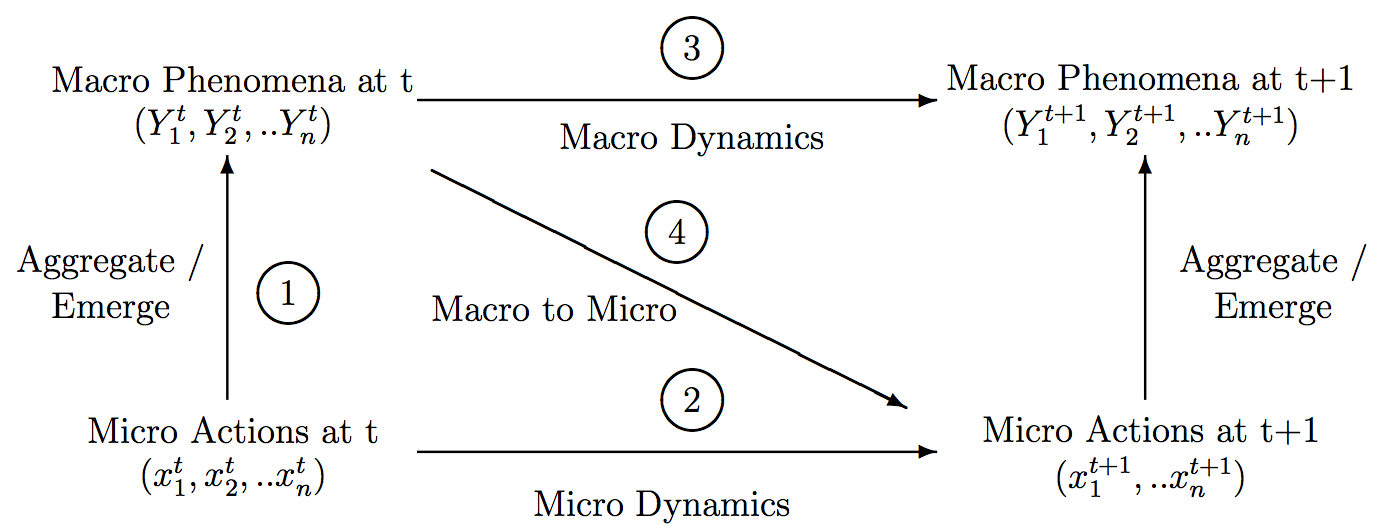
\includegraphics[width=0.9\linewidth]{figuras/micro_macro.png}
    \caption{Interacciones entre micro y macro. Fuente: Page (2015)}
    \label{fig:my_label}
\end{figure} 
\end{frame}

\begin{frame}{Modelos Basados en Agentes}
    \framesubtitle{Algunas aplicaciones en Economía}
    \begin{itemize}
\item Crecimiento: Nelson and Winter (1982), Silverberg, Verspagen, Dosi, Howitt, Llerena and Lorentz (2004); Dawid and Fagiolo (2008); Dosi et al. (2010a); Ciarli et al. (2010); Ciarli (2012); Ciarli et al. (2012); Fagiolo and Roventini (2012).
\item Localización de firmas: David et al. (1998)
\item Cambio tecnológico: Dawid (2006); Teitelbaum and Dowlatabadi (2000); Yildizoglu (2002)
\item Mercados: Axtell, Epstein, Tesfatsion, Kirman and Vriend (2000)
\item Mercado eléctrico: Tesfatsion
\item Estudios sectoriales: Malerba et al
\item Medio ambiente: van den Bergh, Safarzynska, Windrum et al. (2009a,b)
    \end{itemize}
\end{frame}

\begin{frame}{Modelos Basados en Agentes}
    \framesubtitle{(Más) aplicaciones en Economía}
    \begin{itemize}
        \item Ciclos de vida industriales: Windrum and Birchenhall (2005), Malerba et al
\item Mercado de trabajo: Tesfatsion, Fagiolo et al. (2004), Richiardi and Leombruni
\item Mercados financieros: Delli Gatti et al. (2004), Delli Gatti and Stiglitz,  \textit{econophysics}
\item Inestabilidad macro: Bak et al. (1993); Dosi et al. (2006), Weisbuch and Battiston, Ciarli and Valente (2007)
\item Macro: Gallegati, Howitt, Duffy, Arifovic....
\item Coalición de empresas y formación de redes: Cowan and Jonard, Ozman, Page, Huberman, Axtell, Vega-Redondo, Jackson, Watts
\item Otras ciencias sociales: Ciencia Política (cooperación, conflicto), Sociología, Antropología, ...
    \end{itemize}
\end{frame}

\begin{comment}
\begin{frame}{Modelos Basados en Agentes}
    \framesubtitle{Cellular automata}
    \begin{itemize}
\small        \item \textit{``At a very general level, one might say that computation is what a complex system does with information in order to succeed or adapt in its environment.''} Mitchell (2009, ch. 10, p. 146)
\small \item The CA is a kind of complex system where the agents (cell) can change its status or move to another place according to a set of disposal simple rule and depending of the status of its neighborhood. The CA generally is represented in a Lattice (grid) of cells.
    \end{itemize}
   \textcolor{blue}{Game of Life (Conway) and Wolfram Cellular Automata}
    \begin{figure}
        \centering
        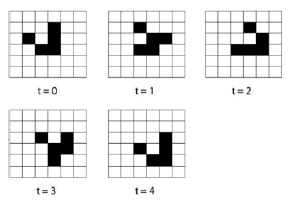
\includegraphics[width=0.25\linewidth]{figuras/conway1.png}
        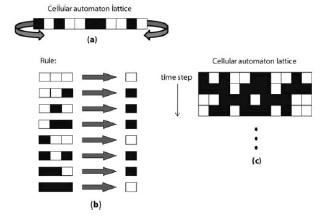
\includegraphics[width=0.25\linewidth]{figuras/conway2.png}
        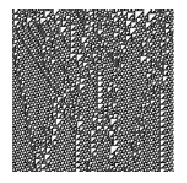
\includegraphics[width=0.25\linewidth]{figuras/conway3.png}
        \label{fig:my_label}
    \end{figure}
\end{frame}

\begin{frame}{Modelos Basados en Agentes}
\framesubtitle{Cellular automata: Game of life}
    \textbf{Rules:}\\
Denoting on cells as alive and off cells as dead, Conway defined the rule in terms of four life processes:
\begin{itemize}
    \item Birth, a dead cell with exactly three live neighbors becomes alive at the next time
step;
\item Survival, a live cell with exactly two or three live neighbors stays alive;
\item Loneliness, a live cell with fewer than two neighbors dies
\item Dead, a dead cell with fewer than three neighbors stays dead
\end{itemize}
\end{frame}
\end{comment}

\begin{frame}{Comparando marcos teóricos}
\framesubtitle{Equilibrio General en pocas líneas}
\begin{multicols}{2}
Supuestos:
\begin{itemize}
  \footnotesize  \item Racionalidad completa (agentes optimizadores completamente informados)
\item Sin tiempo y sin dinámica
\item Solo análisis de equilibrio
\item Sin interacciones (red tipo estrella)
\end{itemize}
Motivación: equilibrio
\begin{itemize}
\footnotesize \item Existencia y singularidad
\item Estabilidad
\end{itemize}
Limitaciones:
\begin{itemize}
 \footnotesize   \item Significado de la existencia de un equilibrio social (¿observación?)
\item ¿Cómo se puede establecer un equilibrio (``subastador'' walrasiano)?
\item ¿Qué sucede fuera del equilibrio (además de la atracción instantánea)?
\item ¿Qué (o quién) es un subastador? ¿Interacciones?
\item ¿Cómo pasa una economía de un equilibrio a otro?
\item ¿Qué sucede en el medio?
\item Supuestos sobre microcomportamiento y poder predictivo (por ejemplo, crisis)
\end{itemize}
\end{multicols}
    
\end{frame}


\begin{frame}{Comparando marcos teóricos}
\framesubtitle{Modelos macro microfundamentados en pocas líneas}
\begin{multicols}{2}
Ejemplo: modelos de crecimiento económico
\begin{itemize}
\footnotesize    \item Empresa representativa con función de producción: $F(L_t , A_t K_t )$
\item Hogar representativo con función de utilidad: $\int_{t=0}^\infty e^{-\rho t} u(C(t)) \dfrac{L_t}{H} dt$
\item Tanto las empresas como los hogares son agentes totalmente racionales (maximizadores), con habilidades computacionales ilimitadas
\end{itemize}
Limitaciones:
\begin{itemize}
    \footnotesize \item Supuestos de racionalidad
\item No hay espacio para la innovación radical y el cambio estructural
\item El cambio agregado en el PIB debe interpretarse como una transición a través de equilibrios (pero el modelo es estático) (Kirman 1989)
\item Heterogeneidad y agregación:
\item[\textcolor{red}{$\rightarrow$}] Las preferencias de un agente representativo sobre las opciones disponibles pueden ser muy diferentes de las de la sociedad
\item[\textcolor{red}{$\rightarrow$}] La reacción de este agente a los shocks no necesariamente refleja cómo reacciona cada individuo a los shocks
\end{itemize}
\end{multicols}
\end{frame}


\begin{frame}{Comparando marcos teóricos}
\framesubtitle{Teoría de Juegos en pocas líneas}
\begin{multicols}{2}
Supuestos:
\begin{itemize}
    \footnotesize \item N agentes con un set de acciones A
\item Pagos: $\Pi (a_i ; a_j , j \neq i)$ (matriz de pagos)
\item Los agentes son completamente racionales.
\item Análisis: Equilibrios de Nash
\item Interacciones: Red completa (vs. red tipo estrella)
\item Ejemplo: Oligopolio con N empresas (Modelo de Cournot)
\end{itemize}
\newpage
Limitaciones:
\begin{itemize}
    \footnotesize \item Supuestos racionales
\item Habilidades computacionales de un agente (¿inducciones hacia atrás? ¿suposiciones sobre el comportamiento de otros agentes?)
\item Problemas cuando N es grande y los juegos se repiten un número finito de veces (problema de regresión)
\item Poder predictivo en juegos repetidos infinitamente
\end{itemize}
\end{multicols}    
\end{frame}

\begin{frame}{Comparando marcos teóricos}
\framesubtitle{¿Realmente necesitamos simulaciones?}
    \begin{itemize}
        \item Depende del fenómeno en estudio.
\item Crisis y regularidades empíricas de los sistemas complejos: las sociedades son complejas.
\item ¿Qué tan razonables y útiles son las suposiciones para lo que queremos estudiar?
    \end{itemize}
\end{frame}

\begin{frame}{Comparando marcos teóricos}
\framesubtitle{¿Realmente necesitamos simulaciones? Aspectos críticos de las simulaciones}
    \begin{itemize}
        \item Las simulaciones producen todo y solo lo que se ingresa en el código
         \begin{itemize}
             \item Es verdad, pero...
             \item las computadoras ayudan a comprender exactamente las implicaciones de las suposiciones.
             \item Emergencia: las computadoras ayudan a llenar el vacío entre las hipótesis y sus implicaciones (por ejemplo, el cambio climático).
         \end{itemize}
\item Validación empírica
\begin{itemize}
     \item La replicación de datos es inútil sin entender su significado.
     \item En primer lugar, es necesario tener pruebas sólidas sobre los supuestos del microcomportamiento
\item Los resultados vienen en forma de distribuciones, dependiendo de la aleatoriedad de las condiciones iniciales y de las interacciones
\end{itemize}
    \end{itemize}
\end{frame}

\begin{frame}{Comparando marcos teóricos}
\framesubtitle{¿Realmente necesitamos simulaciones? Aspectos críticos de las simulaciones}
\begin{itemize}
    \item Prueba de aleatoriedad y espacio de parámetros
     \begin{itemize}
         \item Los modelos aleatorios o los modelos con muchos parámetros deben probarse adecuadamente para determinar la solidez de los resultados: una única ejecución aleatoria puede ser un caso excepcional en una distribución
     \end{itemize}
     \item Cuestiones abiertas cruciales
     \begin{itemize}
         \item Ejercicios de políticas públicas
\item Fomento de técnicas de validación empírica
    \end{itemize}
\end{itemize}
\end{frame}

\begin{comment}
\begin{frame}{Methodology for ABM}
 \framesubtitle{Goals for science}
\begin{itemize}
    \item The goal of science is to increase \underline{knowledge} about real world phenomena.
    \item Scientists generate knowledge by providing \underline{explanations} $A \rightarrow B$ for observed phenomena.
    \item Social sciences frequently concerns non-quantitative phenomena.
\item \underline{Simulation} must be used to \textbf{generate} virtual emergent properties ... and providing \textbf{explanations} for these.
\end{itemize}
\end{frame}

\begin{frame}{Methodology for ABM}
 \framesubtitle{Knowledge as explanations}
Notice the difference between cause and explanation. The
former relates to objective properties of reality, the second to
subjective interpretations.

\vspace{3mm}

\begin{quote}
``Our undertaking is logical rather than ontological. That is, we wish to be able to assert: 'The sentence A stands in a causal relation to the sentence B (in a specified system of sentences)'; and not: 'That which is denoted by sentence A causes that which is denoted by sentence B' ''.\\ \vspace{3mm}
\small Simon, H. A. (1952), On the Definition of the Causal Relation,
\textit{The Journal of Philosophy, 49}(16), pp. 517-528.
\end{quote}
\end{frame}

\begin{frame}{Methodology for ABM}
 \framesubtitle{Knowledge as explanations}
    \begin{itemize}
        \item The definition of knowledge implies also what is not knowledge: pure information, descriptions void of any context. 
\item For example, the description of a system, if not included in an explanation, is not knowledge.
\item A description is necessarily arbitrary, ignoring some aspect and focusing on few ones. The choice of how to describe a state cannot be independent of how the description is used.
    \end{itemize}
\end{frame}
\begin{frame}{Methodology for ABM}
 \framesubtitle{Definitions of knowledge}
 \begin{itemize}
    \item The proposed definition provides some useful indications to
classify research strategies. Since researchers aim at
increasing knowledge, we need to consider how it is possible to
generate new explanations.
There is a surprisingly small number of possible
knowledge-increasing strategies, which may possibly be
combined together.
\end{itemize}   
\end{frame}

\begin{frame}{Methodology for ABM}
 \framesubtitle{Definitions of knowledge}
 \begin{itemize}
  \small      \item Knowledge refinement: An existing explanation, proved
correct on a number of cases, may be proven wrong by a
counter-example. This may be trigger the refining of the
definition of states included in the original (too) general
explanation, or to change the explanatory mechanism, or
simply to throw away the whole piece of knowledge.
\item Knowledge deepening: Knowledge is never ultimately
specified. You can always request a further specification of how
µ is actually working, investigating intermediate steps and their
explanations, potentially diving into infinitely more detailed
explanations.
\item Knowledge extension: Knowledge can be put together
extending existing pieces of knowledge to form chains of
explanations, linking the final state of an explanation to the
initial state of the next
    \end{itemize}
\end{frame}


\begin{frame}{Methodology for ABM}
 \framesubtitle{Implications for research strategy}    
 Research projects should therefore always state explicitly which
class(es) of knowledge they pursue:
\begin{itemize}
    \item Refine: change a currently established conviction.
\item Deepen: provide finer details of an accepted explanation.
\item Extend: link sparse results in a new, unique explanation.
\end{itemize}
Any research project should undergo the following steps:
\begin{itemize}
    \item Start from an established piece of knowledge $A \rightarrow B$
    \item State a conjecture $A \rightarrow B$ which is relevant and novel.
    \item By refining/deepening/extending $A \rightarrow B$, or
\item  ... possibly a new unexpected explanation different from
the initial conjecture.
\end{itemize}
\end{frame}

\begin{frame}{Methodology for ABM}
	\framesubtitle{Verification, validation and calibration} 
	\begin{itemize}
		\item Verification: the process of making sure that the conceptual model matches the implemented model.
\begin{itemize}
\item documentation, testing, case studies and scenarios
\item problems: "bugs", lack of communication, EMERGENCY.
\end{itemize}
\item Validation: the process of making sure that the implemented model matches the real world.
\begin{itemize}
\item "All models are wrong, but some are useful" George E. P. Box
\item Macro-validation: compare the aggregated results
\item Micro-validation: compare individual rules and properties
\end{itemize}
\item Calibration: search for parameters that minimize errors.
	\end{itemize}
\end{frame}

\begin{frame}{Methodology for ABM}
	\framesubtitle{Replication} 
	It is the implementation of a previously described and implemented conceptual model.
\begin{itemize}
\item the results must be replicable to be considered part of scientific knowledge.
\item different dimensions: Hardware, programming languages, algorithms, parameter space.
\item benefits:
\begin{itemize}
\item is gained in knowledge
\item focuses on other problems beyond the original model
\item validation is improved
		\end{itemize}
	\end{itemize}
\end{frame}

\begin{frame}{Methodology for ABM}
 \framesubtitle{Assessment}  
 We call a model an implementation of a piece of knowledge, where symbols and their relations express the knowledge
content.
The assessment of a model can be divided in three phases:
\begin{itemize}
    \item Descriptive relevance (abstraction). The choice of the symbolic representation for the reality of interest.
\item Internal consistency (verification). Manipulation of symbols to generate conclusions from observation and assumptions.
\item Results’ relevance (validation). The assessment of the results as compared to empirical observations.
\end{itemize}
\end{frame}

\begin{frame}{Methodology for ABM}
 \framesubtitle{Research strategy}  
 \begin{figure}
       \centering
       \includegraphics[width=0.8\linewidth]{figuras/Captura desde 2022-09-20 02-51-44.png}
       \label{fig:my_label}
   \end{figure} 
\end{frame}


\begin{frame}{Methodology for ABM}
\framesubtitle{Objectivity}
   No universal objective criterion can ever be devised to
objectively assess a model.
   \begin{enumerate}
       \item Descriptive relevance (abstraction). The choice of the
symbolic representation can always be questioned in
principle. \textbf{Subjective}.
\item Internal consistency (verification). The derivation of the
consequences from the assumptions can be \textbf{objectively}
evaluated. However whether the modeled mechanism are
compatible with the real ones remain \textbf{subjective}.
\item Results’ relevance (validation). Results adherence to
reality is potentially questionable, as any piece of reality is
context- and history-dependent. \textbf{Subjective}
   \end{enumerate}
\end{frame}

\begin{frame}{Methodology for ABM}
\framesubtitle{Explanation assessment}    
How to assess a proposed model depends on the nature of the
phenomenon under study.\\
There are two classes of phenomena:
\begin{itemize}
    \item Quantitative: phenomena defined by a constant vector of
variables and explained by mathematical operations. 
\item Qualitative: phenomena defined by a varying number of
non-quantitative aspects logically, but not quantitatively,
explained.
\end{itemize}
\end{frame}

\begin{frame}{Methodology for ABM}
\framesubtitle{Quantitative phenomena}
Quantitative phenomena express explanations as functions
linking a fixed set of variables:
\begin{equation*}
    y=f(x)
\end{equation*}

Hence, assessment can be performed by simple comparison
between theoretical and empirical data:
\begin{enumerate}
    \item collect samples of empirical data $X^*$ and $Y^*$
    \item compute the expected data $Y'=f(X^*)$
\item compute the error $|Y'-Y^*|$
\end{enumerate}
Assessment can therefore be reduced to measure the size of the error.
\end{frame}

\begin{frame}{Methodology for ABM}
\framesubtitle{Qualitative phenomena}
 \begin{itemize}
     \item Qualitative phenomena consist in dynamics of entities that
cannot be represented by a fixed and constant set of variables:
emergent properties.
\item The elements of the system, though clearly identifiable, change
not only in the intensity of certain measures, but also the very
relevant measures.
\item Quantitative aspects for qualitative phenomena do exist, in
general, and are highly relevant. However, these measures are
not the phenomenon, but only proxies and partial
representations of the actual phenomenon, whose significance
goes beyond its quantitative measures.
\item On the contrary, quantitative phenomena are made of the very
measures.
 \end{itemize} 
\end{frame}

\begin{frame}{Methodology for ABM}
\framesubtitle{Qualitative phenomena}
   General features for qualitative phenomena are:
   \begin{itemize}
        \item Structurally dynamic: varying number of variables/measures relevant to describe entities involved.
\item Open systems: heavily influenced by a non-neutral environment.
    \end{itemize}
As a consequence, qualitative phenomena are:
\begin{itemize}
    \item Highly sensitive to small deviations in initial conditions.
\item High number of idiosyncratic features.
\item Strongly path-dependent.
\end{itemize}
\end{frame}


\begin{frame}{Methodology for ABM}
\framesubtitle{Qualitative phenomena}
ABM are uniquely able to express qualitative phenomena since
it can express all the three components of explanations:
\begin{itemize}
    \item Aggregate explanations: model data structure can
represent complex non linear hierarchical relations.
\item Temporal explanations: irreversible time constraints
forced by the structure of the programming language.
\item Logical explanations: unlimited set of possible
computational structures.
\end{itemize}

An ABM can therefore be used to replicate not (only) the state
of a system, but the very explanations linking its states.
\end{frame}


\begin{frame}{Methodology for ABM}
\framesubtitle{Qualitative phenomena}
Using a model to target a \textbf{qualitative} phenomenon should follow
this procedure:
\begin{enumerate}
    \item Define a research question in terms of a conjectured
explanation.
\item Implement the elements relevant for the phenomenon.
\item Ensure that the overall result is compatible with available
evidence (replicate the emergent property).
\item Identify how the results are generated: verify the model.
\item Compare the explanations for the simulated events with
those in real systems.
\end{enumerate}
The advantage of ABM is to allow the investigation of \textbf{how} a
well-specified phenomenon occurs.
\end{frame}

\end{comment}

\begin{frame}{Metodología para ABM}
\framesubtitle{Pasos a seguir en un ABM}
\begin{enumerate}
    \item Escribir el modelo: definir la estructura de datos, sus valores iniciales y su dinámica.
\item Analizar los resultados: asegurarnos que los resultados finales puedan interpretarse como las propiedades emergentes objetivo.
\item Debug: investigar las motivaciones por las cuales el modelo genera los resultados.
\item Documentar: validar la supuesta explicación encontrando apoyo empírico que demuestre que esas explicaciones también funcionan en la realidad.
\item Refinar: ampliar el modelo modificando la estructura de datos y/o las condiciones iniciales y/o la dinámica. Volver al paso 2.
\end{enumerate}
\end{frame} 

\begin{frame}{Metodología para ABM}
\framesubtitle{Pasos a seguir en un ABM (G. Silverberg)}
    \begin{figure}
        \centering
        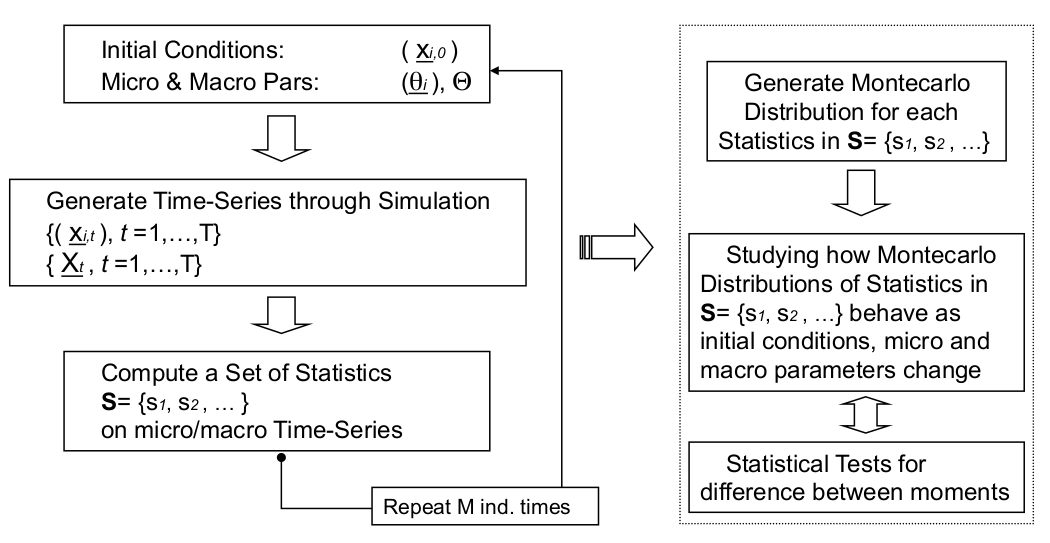
\includegraphics[width=0.9\linewidth]{figuras/Captura desde 2022-09-21 11-57-19.png}
    \end{figure}
\end{frame}

\begin{frame}{Metodología para ABM}
\framesubtitle{Pasos a seguir en un ABM: refinamientos}
 \begin{itemize}
     \item  En los modelos, como en los sistemas económicos, es muy probable que la mayoría de los elementos interactúen, directa o indirectamente, con la mayoría de los demás. Los efectos de las interacciones en los resultados del modelo son difíciles de predecir e imposibles de corregir.
\item Construir un modelo complejo completo desde cero corre el riesgo de caer en una \textbf{trampa de complejidad}: no poder asociar las propiedades de los resultados a las características del modelo. En este caso el modelo se vuelve inútil, porque son estas asociaciones las que aportan nuevos conocimientos.
 \end{itemize}  
\end{frame}

\begin{frame}{Metodología para ABM}
\framesubtitle{Pasos a seguir en un ABM: refinamientos}
\begin{itemize}
\small    \item Para evitar esto, es necesario desarrollar un modelo gradualmente, a partir de prototipos simples y avanzando un paso por vez. 
\item En cada paso, introduce una modificación y espera un efecto determinado en los resultados. Si se cumplen las expectativas, puede proceder con seguridad. De lo contrario, puede comenzar desde el último paso para revisar el modelo.\\
\item Entonces, un paso en la revisión del modelo puede tomar una de las tres formas de creación de conocimiento:
\begin{itemize}
\small \item \textbf{Revisión de conocimientos:} modificar una función o la estructura de un sistema para corregir resultados no deseados.
\item \textbf{Profundización del conocimiento:} endogenizar elementos de un modelo existente, por ejemplo, convertir una variable que representa una función de demanda en un modelo de consumidores.
\item \textbf{Ampliación del conocimiento:} agregar nuevos elementos a un modelo, o fusionar dos modelos diferentes en uno solo.
\end{itemize}
\end{itemize}
\end{frame}

\begin{frame}{Metodología para ABM}
    \framesubtitle{Aprendizaje}
    \begin{itemize}
        \item \textbf{Aprender escribiendo código:} la necesidad de representar computacionalmente un sistema obliga a pensar cómo funcionan realmente los sistemas reales.
\begin{itemize}
     \item Un modelo es un universo simulado, con las mismas restricciones lógicas que el real.
\item Las representaciones aparentemente obvias resultan ser inconsistentes o incompletas cuando se intentan codificar.
\item Encontrar la manera correcta de expresar mediante un lenguaje formal una síntesis de un sistema real proporciona muchos conocimientos sobre el sistema mismo.
\end{itemize}
\item \textbf{Aprender mediante gráficos:} el análisis de los resultados (a lo largo del tiempo y/o diferentes inicializaciones) proporciona evidencia del comportamiento del modelo.
\begin{itemize}
     \item Controlar que su modelo produzca fenómenos realistas genera una nueva comprensión de los casos reales, sus características y otras propiedades no obvias a partir de la observación del mundo real.
\end{itemize}
    \end{itemize}
\end{frame}

\begin{frame}{Metodología para ABM}
    \framesubtitle{Aprendizaje (cont.)}
    \begin{itemize}
        \item \textbf{Depurando código:} vincular lógicamente el contenido del modelo con los resultados producidos por las simulaciones proporciona una perspectiva sorprendente, que muestra consecuencias no obvias del diseño y la implementación del modelo. Estas explicaciones incorporan el conocimiento definitivo sobre el sistema simulado, con suerte válido también para los reales.
\item \textbf{Cometiendo errores:} Los errores en el diseño de los modelos de simulación reflejan conceptos erróneos. La generación de errores muestra las consecuencias de las fallas originales, y con frecuencia sugiere soluciones y mejoras.
    \end{itemize}
\end{frame}
\end{document}